\section{Auswertung}

In dem Versuch wird ein Acryblock untersucht. Dieser Block hat folgende Maße:
\begin{gather*}
	\text{Länge: 15 cm} \\
	\text{Höhe: 8 cm}\\
	\text{Dicke: 4 cm}\\
\end{gather*}
Zudem haben die verwendeten Sonden jeweils eine Schutzschicht mit der Dicke
\begin{equation*}
	D = 0,2 \text{cm}
\end{equation*}

\subsection{Untersuchung mit A-Scan}
\label{subsec:A-Scan}

Mithilfe des A-Scans werden für die Löcher 3 bis 10 folgende Werte ermittelt, zu sehen in Tabelle \ref{tab:1.1}:

\begin{table}[h!]
\centering
\caption{Ergebnisse des A-Scans.\label{tab:1.1}}
	\begin{tabular}{c|c|c}
		\toprule
		{$n_\text{Loch}$} & {$t1 / \text{\mu s}$} & {$t2 / \text{\mu s}$}\\
		\hline
        	\midrule
	3& 46.5 &9.7\\
	4 &40 &15.9\\
	5 &34.6 &22.1\\
	6 &29.1 &28.4\\
	7 &23.4 &34.1\\
	8 &17.6 &39.9\\
	9 &11.7 &45.6\\
	10 &5.7 &51.7\\
	\bottomrule 
	\end{tabular}
\end{table}

$t1$ und $t2$ sind dabei die Laufzeiten von der jeweiligen Seite des Blocks. Nach Gleichung \ref{eq:3} und Abzug der Dicke der Schutzschicht ergeben sich die Positionen der Löcher im Block, bzw. die Distanz von der Messwand.
Die Geschwindigkeit $c$, die Schallgeschwindigkeit, beträgt in Acryl 2730 m/s \cite{2}.
Mit der Rechnung
\begin{equation}
	G_\text{Loch} = h_\text{Block} - S_2 - S_1
\end{equation}
ergibt sich dann die Größe der Löcher (Tabelle \ref{tab:12}).  $S_1$ und $S_2$ sind jeweils die Strecken-Messungen von 'oben' und 'unten' des Blockes. 

\begin{table}[H]
\centering
\caption{Laufwege }
\label{tab:12}
	\begin{tabular}{c|c|c|c}
		\toprule
		{$N_\text{Loch}$} & {$S_1 / \text{cm}$} & {$S_2 / \text{cm}$} & {$G_\text{Loch} / \text{cm}$}\\
		\hline
        	\midrule
	3&6.15&1.12&0.73 \\
	4 &5.26&1.97&0.77\\
	5 &4.52&2.82&0.66\\
	6 &3.77&3.68&0.55\\
	7 &2.99&4.45&0.55\\
	8 &2.20&5.25&0.55\\
	9 &1.40&6.02&0.58\\
	10 &0.58&6.86&0.56\\
	\bottomrule 
	\end{tabular}
\end{table}

\subsection{Auflösungsvermögen}


Für die Messfrequenzen 1 MHz (Abbildung \ref{fig:1MHz}), 2 MHZ (Abbildung \ref{fig:2MHz}) und 4 MHz (Abbildung \ref{fig:4MHz}) ergeben sich folgende Graphen bei der Untersuchung des Acrylblocks.

 \begin{figure}[H]
		\centering
		\includegraphics[scale=0.5]{Auswertung/1MHz-Auflösung.png}
		\caption{Auflösung bei 1 MHz.}
		\label{fig:1MHz}
\end{figure}
\begin{figure}[H]
		\centering
		\includegraphics[scale=0.5]{Auswertung/2MHz-Auflösung.png}
		\caption{Auflösung bei 2 MHz.}
		\label{fig:2MHz}
\end{figure}
 \begin{figure}[H]
	\centering
	\includegraphics[scale=0.5]{Auswertung/4MHz-Auflösung.png}
	\caption{Auflösung bei 4 MHz.}
	\label{fig:4MHz}
\end{figure}

An den Graphen ist erkennbar, dass bei 4 MHz die höchste Auflösung besteht und bei 1 MHz die geringste. Bei 4 MHz sind die Peaks der beiden Löcher klar erkennbar. Bei 1 MHz sind sie nicht mehr differenzierbar. 

\subsection{Untersuchung mit B-Scan}

Bei der Messung mithilfe des B-Scans ergeben sich folgende Abbilder des Acrylblocks (oben / unten):
 \begin{figure}[H]
		\centering
		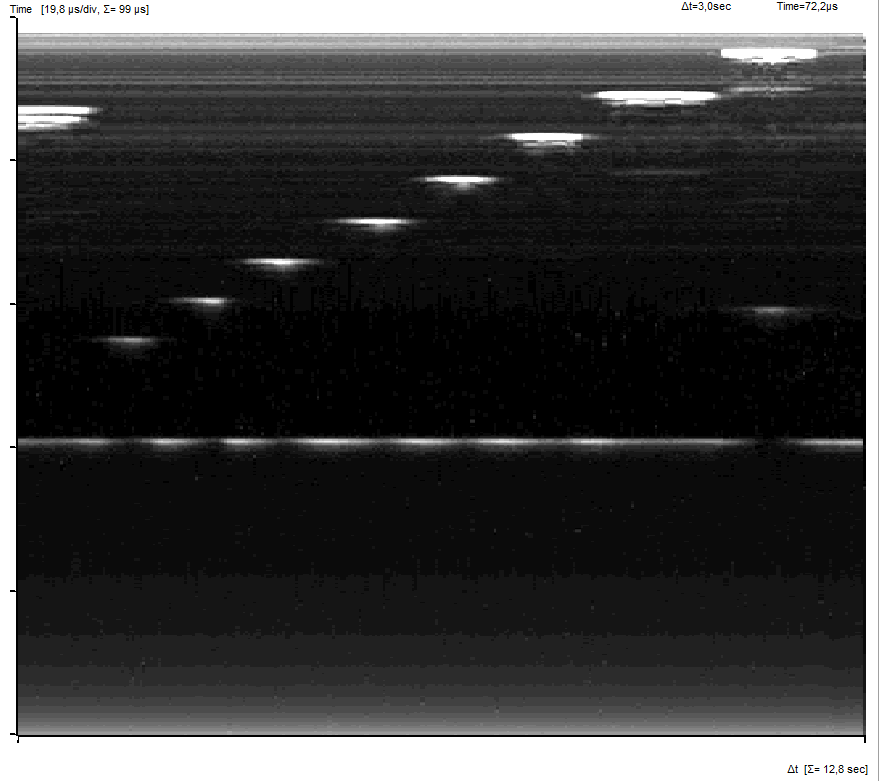
\includegraphics[scale=0.4]{Auswertung/B-Mode.png}
		\caption{Abbild des Acrylblocks mit B-Scan (oben).}
		\label{fig:B1}
\end{figure}
\begin{figure}[H]
		\centering
		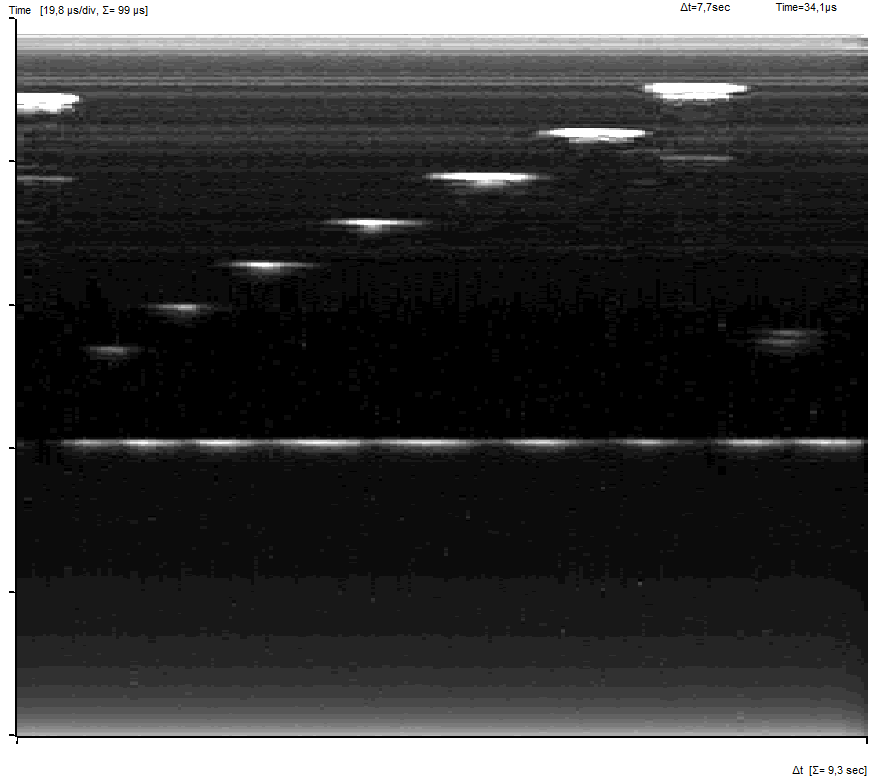
\includegraphics[scale=0.4]{Auswertung/B_Mode2.png}
		\caption{Abbild des Acrylblocks mit B-Scan (oben).}
		\label{fig:B2}
\end{figure}

Wie beim A-Scan \ref{subsec:A-Scan} können nun erneut mithilfe Gleichung \ref{eq:3} die jeweiligen Laufwege über die Laufzeiten (siehe Tab. \ref{tab:T2}) bestimmt werden. 
\begin{table}[H]
\centering
\caption{Laufzeiten beim B-Scan. }
\label{tab:T2}
	\begin{tabular}{c|c|c|c|c}
		\toprule
		{$N_\text{Loch}$} & {$t_{1,1} / \text{\mu s}$} & {$t_{2,1} / \text{\mu s}$} & {$t_{1,2} / \text{\mu s}$} & {$t_{2,2} / \text{\mu s}$}\\
		\hline
        	\midrule
	1&15.7&16.8&46.4&47.1\\
	2&14.3&15.5&45.0&46.0\\
	3&46.0&47.1&10.8&13.2\\
	4&40.7&41.7&17.0&19.1\\
	5&35.2&36.3&23.2&25.3\\
	6&29.6&31.0&29.6&31.8\\
	7&23.8&25.3&35.6&36.9\\
	8&17.7&19.5&41.3&43.0\\
	9&12.1&14.3&47.1&48.3\\
	10&6.1&8.2&---&---\\
	11&41.7&43.2&12.2&15.1\\
	\bottomrule 
	\end{tabular}
\end{table}
Die Größen der Löcher werden mithilfe der Gleichung 
\begin{equation}
	G_\text{Loch} = S_{2,n} - S_{1,n}
\end{equation}
berechnet (sieh Tab. \ref{tab:G2}).
 
\begin{table}[H]
\centering
\caption{Laufwege und Größen der Löcher beim B-Scan.}
\label{tab:G2}
	\begin{tabular}{c|c|c|c|c|c|c}
		\toprule
		{$N_\text{Loch}$} & {$S_{1,1} / \text{cm}$} & {$S_{2,1} / \text{cm}$} &  {$S_{1,2} / \text{cm}$}& {$S_{2,2} / \text{cm}$} &{$G_\text{Loch,1} / \text{cm}$}&{$G_\text{Loch,2} / \text{cm}$}\\
		\hline
        	\midrule
	1&1.94&2.09.&6.13&6.23&0.15&0.10\\
	2&1.75&1.92&5.94&6.08&0.16&0.14\\
	3&6.08&6.23&1.27&1.60&0.15&0.33\\
	4&5.36&5.49&2.12&2.41&0.14&0.29\\
	5&4.60&4.75&2.97&3.25&0.15&0.29\\
	6&3.84&4.03&3.84&4.14&0.19&0.30\\
	7&3.05&3.25&4.66&4.84&0.20&0.18\\
	8&2.22&2.46&5.44&5.67&0.25&0.23\\
	9&1.45&1.75&6.23&6.39&0.30&0.16\\
	10&0.63&0.92&---& --- &0.29&---\\
	11&5.49&5.70&1.47&1.86&0.20&0.40\\
	\bottomrule 
	\end{tabular}
\end{table}

$n$ steht dabei für die jeweilige Seite auf der der Block bei der Messung liegt, \\ also oben/unten. Bei $n = 1$ sind die beiden kleinen Löcher oben.

\subsection{Herzmodell mit TM-Scan}

Bei der Messung eines A-Scans des Herzmodelles ergibt sich eine Echolaufzeit von
\begin{equation*}
	t = 53,5 \text{\mu s}   .
\end{equation*}

Bei dem TM-Scan werden 8 Peaks aufgenommen über eine Zeit von 9,6 s (siehe Abbildung \ref{fig:TM}).
 \begin{figure}[H]
	\centering
	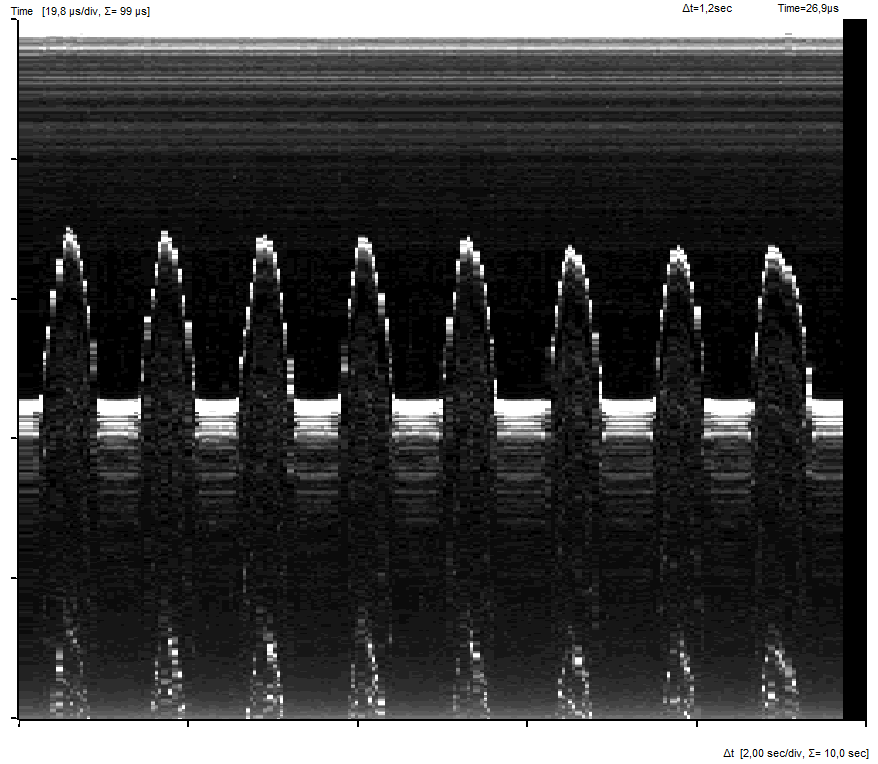
\includegraphics[scale=0.4]{Auswertung/Herz.png}
	\caption{TM-Scan eines Herzmodells.}
	\label{fig:TM}
\end{figure}
Somit ergibt sich nach 
\begin{equation*}
	f = \frac{t}{n} \cdot 60
\end{equation*}
eine Herzfrequenz von 76 Schlägen pro Minute.

Die Peaks verlaufen jeweils zeitlich von 32,8 \mu s bis 55,9 \mu s. 
\\
Das Herzmodell hat einen Durchmesser von 5 cm und kann als Halbkugel betrachtet werden. 
Bei dem Enddiastolischen Volumen, kurz EDV, handelt es sich um das Blutvolumen, welches nach maximaler Füllung in einer Herzkammer vorzufinden ist. Somit kann über die Echolaufzeit mit der Gleichung \ref{eq:3} das Volumen des Modells ohne Kontraktion des Ballons (Herz) bestimmt werden. 
Die Geschwindigkeit $c$, die Schallgeschwindigkeit, beträgt in Wasser 1484 m/s.
Das Volumen eines Zylinders ist definiert als
\begin{equation*}
	V_\text{Z} = \pi \cdot r^2 \cdot h  .
\end{equation*}
$h$ ist definiert als s aus \ref{eq:3}.
Für das Modellherz ergibt sich also eine Enddiastolisches Volumen von 
\begin{equation*}
	\text{EDV} = 157.08 \text{ml} .
\end{equation*}
Das Endsystolische Volumen, kurz ESV, gibt das Blutvolumen nach voller Kontraktion des Herzens in einer Herzkammer an. Somit muss dem Volumen des voll aufgespannten Herzens, hier Ballons, das zuvor berechnete Volumen abgezogen werden.
Für das vom Herzen eingenommenen Volumen wird die Gleichung
\begin{equation*}
	V_\text{Halbkugel} = \frac{2}{3} \cdot \pi \cdot r^3
\end{equation*}
verwendet.
Für das Endsystolische Volumen ergibt sich somit
\begin{equation*}
	\text{ESV} = 104.72 \text{ml}
\end{equation*}

Zur Bestimmung des HZV wird nun das ESV vom EDV abgezogen und mit der Herzfrequenz multipliziert:
\begin{equation*}
	\text{HZV} = (\text{EDV} - \text{ESV}) \cdot f
\end{equation*}
Somit ergibt sich ein Herzzeitvolumen von
\begin{equation*}
	\text{HZV} = 3979 \frac{\text{mL}}{\text{min}}
\end{equation*}
	


